\chapter{Method}\label{cha:method}
This chapter motivates the proposed system and derives a formal
description of the proposed trajectory model from the problem of
predicting arrival times by comparing trajectories. 
It then describes the implementation details of the model, and what
approximations and simplifications that have been made.

\section{Model derivation}
Conceptually, the model assumes that similar trajectories, with
respect to their motion patterns, should arrive at 
approximately the same time. When presented with a new trajectory, the system
finds previously observed trajectories with similar motion patterns,
and predict arrival times based on the most similar ones. 

To find similar trajectories, a trajectory similarity metric 
is needed. Additionally, it need to be well defined for
trajectories of different temporal lengths, and unevenly
distributed observations. One way to define a local similarity metric from
an observed trajectory $\traj_{i}$ to trajectory $\traj_{j}$ 
is as the sum of distances of orthogonal
projections onto $\traj_{j}$, as illustrated in Figure~\ref{fig:trajectory-projection}.
\begin{figure}
  \centering
  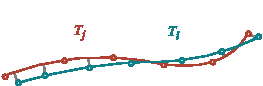
\includegraphics[scale=2.5]{trajectory-projection}
  \caption{An illustration of local distances from $\traj_i$ to
  $\traj_j$ as point-wise orthogonal projections.}\label{fig:trajectory-projection}
\end{figure}
This approach would eliminate the need to align observations before
comparison. However, it requires a continuous trajectory
representation, even though trajectories are observed as discrete samples.
Seeing the observations as samples from a continuous function
$\traj_{k} = \tilde{f}_{k}(t)$ gives a description the trajectory as a function of
time, which is indeed continuous. However, this description is based on specific time
points, but the \textit{exact points in time} of observations are not
relevant, since trajectories for a single segment are generated at many different
occasions. Instead, observations are modeled as samples from a function
$\traj_{k} = \bar{\modelf}_{k}(\synchspace)$, where $\synchspace = [0, 1]$ 
is the \textit{progress} from start ($\synchspace = 0.0$) to finish ($\synchspace = 1.0$) 
of a trajectory. This function models observations based on
progression for any trajectory, regardless of the exact observation
time points.

The function $\bar{\modelf}_{k}$ maps values in $\synchspace$ to 
a state vector of observed positions and velocities $p_x, p_v, v_x, v_y$.
However, modeling a function which takes a scalar to a vector as a GP
would require dependent outputs, which complicates computations considerably. 
Instead $\bar{\modelf}_{k}$ is assumed to be a family of four functions
$\modelf_{k} = (\modelf^{(k)}_{p_x}, \modelf^{(k)}_{p_y}, \modelf^{(k)}_{v_x}, \modelf^{(k)}_{v_y})$
which maps the corresponding dimensions of the state vector.
Independent GP priors are assumed for each function, which gives
\begin{equation}
  \label{eq:f-posterior}
  \begin{split}
  p_x \vert \synchspace \sim & \mathcal{N}(\mu_{p_x}, \Sigma_{p_x}), \\
  p_y \vert \synchspace \sim & \mathcal{N}(\mu_{p_y}, \Sigma_{p_y}), \\
  v_x \vert \synchspace \sim & \mathcal{N}(\mu_{v_x}, \Sigma_{v_x}), \\
  v_y \vert \synchspace \sim & \mathcal{N}(\mu_{v_y}, \Sigma_{v_y}).
  \end{split}
\end{equation}

\begin{figure}
  \centering
  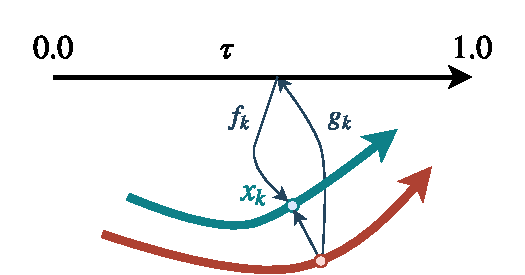
\includegraphics[scale=0.8]{model-projection-perspective}
  \caption{Conceptual illustration of finding the orthogogonal
    projection $x_k$ onto trajectory $\traj_k$ from observation $x$
    through the composition of $f_k \circ g_k$.}\label{fig:model-projection-concept}
\end{figure}
Finding a projection for an observation $\newobs$ onto trajectory
$\traj_{k}$ can now be seen as finding how far along the trajectory $\newobs$
would have traveled. More precisely, finding the $\synchspace$ that $\newobs$
corresponds to, which can then be taken through $\modelf_{k}$
to get the projection.
%% \begin{figure}
%%   \centering
%%   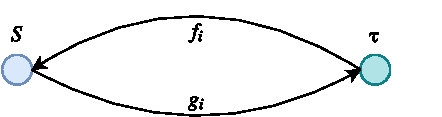
\includegraphics[scale=1.5]{synch-model}
%%   \caption{An illustration of the mappings involved when synchronising
%%     trajectories. Trajectories are observed in the \textit{state space} $\statespace =
%% (p_x, p_y, v_x, v_y)$, containing position and velocity. Then projected by $p$ onto the
%%     subspace $\posspace = (p_x, p_y)$. Then onto
%%     $\synchspace$ by $\synchf_{k}$, and finally back onto $\statespace$ by
%%     $\modelf_{k}$.}\label{fig:synch-model}
%% \end{figure}
To find the corresponding $\synchspace$ to $\newobs$ the inverse of
a mapping from state to $\synchspace$ $\synchf_{k}$ is required. However, when considering progress along a segment,
the current velocity does not matter, and so $\synchf_{k}$ only depends on $(p_x, p_y$).
A GP prior is assumed for $\synchf_{k}$ which gives 
$\synchspace \vert \newobs \sim \mathcal{N}(\mu_{\synchspace}, \Sigma_{\synchspace})$.
The projection onto $\traj_{k}$ can now be computed through the composition 
of the estimated functions $\stochobs_{k} = (\modelf_{k} \circ \synchf_{k})(\obs)$, 
illustrated in Figure~\ref{fig:model-projection-concept}. 
While this approach serves as good intuition, it does not consider the uncertainty in
the estimated functions or observations. To do this, a probabilistic approach is needed, where the
similarity metric of a trajectory is seen as the probability of the corresponding
synchronisation model. The probability of a model is given by Bayes theorem
\begin{equation}
  \label{eq:model-posterior-probability}
  \prob(\synchmodel_{k} \vert \stochobs_{k} = \newobs, \stochobs_{obs} = \newobs) \propto
  \prob(\stochobs_{k} = \newobs \vert \stochobs_{obs} = \newobs, \synchmodel_{k})
  \prob(\synchmodel_{k}),
\end{equation}
for a uniform prior, where $\stochobs_{obs}$ is a stochastic variable for observations,
$\stochobs_{k}$ is a stochastic variable for the
projection. The likelihood is given by
\begin{equation}
  \label{eq:model-likelihood}
  \prob(\stochobs_{k} = \newobs \vert \stochobs_{obs} = \newobs, \synchmodel_{k}) =
  \int \prob(\stochobs_{k} = \newobs \vert \synchspace, \synchmodel_{k}) 
  \prob(\synchspace \vert \stochobs_{obs} = \newobs, \synchmodel_{k}) d\synchspace,
\end{equation}
where $\prob(\stochobs_{k} = \newobs \vert \synchspace,
\synchmodel_{k})$ and $\prob(\synchspace \vert \stochobs_{obs} = \newobs,
\synchmodel_{k})$ are given by equations~\ref{eq:gp},~\ref{eq:gp-mean-function},
and~\ref{eq:gp-covariance-function} for the GPs modeling
$\modelf_{k}$ and $\synchf_{k}$ respectively. This properly expresses
the probability of a model given an observation.

The final piece is to make arrival time predictions. Predicting the
arrival time to the next stop can be seen as 
learning the remaining time of a segment $\arrtime_{k}$ given a point in progression $\synchspace$.
Since time is naturally smooth, a GP prior is assumed for the function 
$\arrtime_{k} = \predf_{k}(\synchspace)$. This gives 
\begin{equation}
  \label{eq:arrival-time-probability}
  \prob(\arrtime_{k} \vert \stochobs_{obs} = \newobs, \model_k) 
  = \int \prob(\arrtime_{k} \vert \synchspace,
  \model_{k}) \prob(\synchspace \vert \stochobs_{obs} 
  = \newobs, \model_{k}) d\synchspace,
\end{equation}
where $\prob(\arrtime_{k} \vert \stochobs_{obs} = \newobs, \model_k)$
and $\prob(\synchspace \vert \stochobs_{obs} = \newobs,
\synchmodel_{k})$ are given by equations~\ref{eq:gp},~\ref{eq:gp-mean-function},
and~\ref{eq:gp-covariance-function} for the GPs modeling
$\predf_{k}$ and $\synchf_{k}$ respectively. 
The trajectory model $\model_{k}$ for trajectory $\traj_k$ is given by the triple 
$\model_{k} = (\modelf_{k}, \synchf_{k}, \predf_{k})$, and
the final model $\model$ is given by the set of 
trajectory models for all $K$ previously observed trajectories, as
illustrated in Figure~\ref{fig:deep-gp-model}.
\begin{figure}
  \centering
  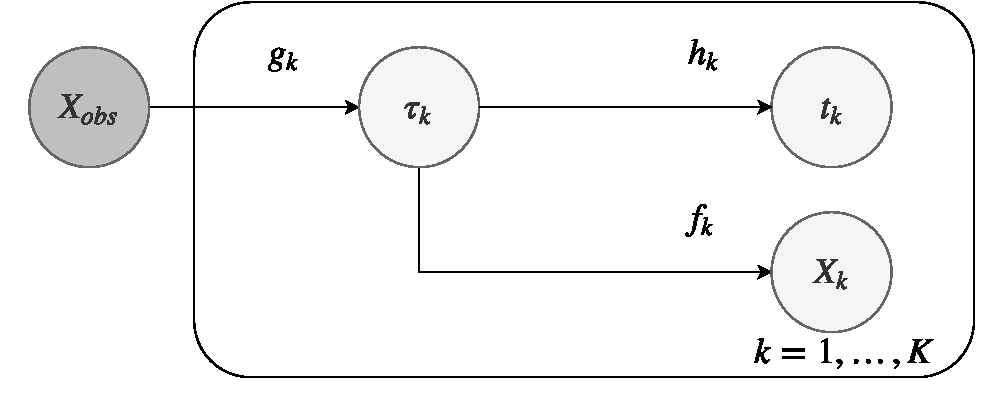
\includegraphics[scale=0.8]{deep-gp-model-2}
  \caption{The model in plate notation.}\label{fig:deep-gp-model}
\end{figure}

\subsection{Approximating the mapping onto $\synchspace$}
The integrals in equations~\ref{eq:arrival-time-probability} and
~\ref{eq:model-likelihood} have no closed form solutions.
Although they can be approximated by using sampling algorithms,
those are computationally expensive. To
avoid this, the likelihood is approximated as
$\delta_{\mu_{\synchspace}}$, that is, a Dirac delta function at the
mean prediction. Intuitively, this approximation discards the variance
of the distribution, treating it as a point-estimated value.
This simplifies equation~\ref{eq:arrival-time-probability} to
\begin{equation}
  \begin{split}
    \prob(\stochobs_{k} = \newobs \vert \stochobs_{obs} = \newobs,
    \synchmodel_{k}) & = 
    \int \prob(\stochobs_{k} = \newobs \vert \synchspace, \synchmodel_{k}) 
    \prob(\synchspace \vert \stochobs_{obs} = \newobs,
    \synchmodel_{k}) d\synchspace \\
    & = \int \prob(\stochobs_{k} = \newobs \vert \synchspace, \synchmodel_{k}) 
    \delta_{\mu_{\synchspace}} d\synchspace \\
    & = \int \prob(\stochobs_{k} = \newobs \vert \synchspace, \synchmodel_{k}) d\synchspace
    \times \int \delta_{\mu_{\synchspace}} d\synchspace = \\
    & = \int \prob(\stochobs_{k} = \newobs \vert \synchspace,
    \synchmodel_{k}) d\synchspace \times 1 = \\
    & = \int \prob(\stochobs_{k} = \newobs \vert \synchspace,
    \synchmodel_{k}) d\synchspace,
  \end{split}
\end{equation}
through the linearity of the integral operator and the property
\begin{equation}
  \label{eq:dirac-integral}
  \int_{-\infty}^{\infty} \delta_{\mu_{\synchspace}} = 1,
\end{equation}
of the Dirac delta function. The resulting integrand is Gaussian
so the integral has a closed form solution, and can be computed
efficiently. Equation~\ref{eq:model-likelihood} is in the same way
simplified to
\begin{equation}
  \begin{split}
    \prob(\arrtime \vert \stochobs_k = \newobs, \model_{k}) =
    \int \prob(\arrtime_k | \synchspace, \tilde{\model}_k) \delta_{\mu_{\synchspace}} d\synchspace
  \end{split}
\end{equation}

%extending the synchronisation model to the \textit{trajectory model}
%$\model_{k} = (\modelf_{k}, \synchf_{k}, \predf_{k})$, illustrated in Figure~\ref{fig:trajectory-model}.
%% \begin{figure}
%%   \centering
%%   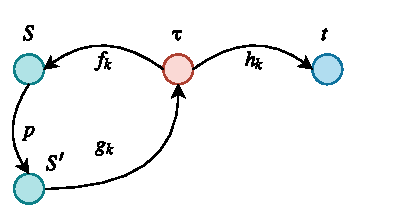
\includegraphics[scale=1.5]{trajectory-model}
%%   \caption{An illustration of the trajectory model, which models
%%     current state $\statespace$ and time left $\arrtime$ as functions of
%%     progress $\synchspace$. New trajectories are observed in 
%%     $\statespace = (p_x, p_y, v_x, v_y)$, containing position and velocity. 
%%     $p$ denotes orthogonal projection onto the subspace $\posspace = (p_x,
%%     p_y)$, which is the domain of $\synchf_{k}$. Via $p$,
%%     $\synchf_{k}$ gives the progression $\synchspace$ of an
%%     observation. The projection onto a trajectory for some $\synchspace$ is given
%%     by $\modelf_{k}$, which is used to compute the data
%%     likelihood. Finally, arrival time predictions are made through $\predf_{k}$.}\label{fig:trajectory-model}
%% \end{figure}


%An illustration of the mappings involved when synchronising
%    trajectories. 
% When trajectories are seen from the same
% $\synchspace$ (that is, they have been mapped over the same $\synchf$),
% through their models $\modelf$, they are
% synchronised. Hence the tuple $\synchmodel_{k} = (\modelf_{k},
% \synchf_{k})$ is referred to as the \textit{synchronisation model}.

% taking the exponent of the data log likelihood
% \begin{equation}
%   \label{eq:model-log-likelihood}
%   \begin{split}
%     \log P(\synchspace \vert \stochobs_{obs} = \newobs, \synchmodel_{k})
%     & = -\frac{1}{2}(\synchspace - \mu(\newobs)){[\Sigma(\newobs)]}^{-1}(\synchspace - \mu(\newobs)) \\
%     & = -\frac{1}{2}\log{|\Sigma(\newobs)|}+C,
%   \end{split}
% \end{equation}
% where $\mu(\newobs)$ and $\Sigma(\newobs)$ are given by
% equations~\ref{eq:gp-mean-function},
% and~\ref{eq:gp-covariance-function} for a GP modeling $f_{k}$. 

% %The likelihood measures how well $\synchmodel_{(k)}$ explains observation
% %$\newobs$, and is a measure of similarity. Assuming that all models
% %are equally probable a priori, Bayes theorem gives
% \begin{equation}
%   \label{eq:model-posterior}
%     P(\synchmodel_{synch}^{(k)} \vert \newobs, \synchspace)
%      \propto P(\synchspace \vert \newobs, \synchmodel_{synch}^{(k)})  
%     P(\synchmodel_{synch}^{(k)}) 
%     \propto P(\synchspace \vert \newobs, \synchmodel_{synch}^{(k)})
% \end{equation}
% and the most similar model can consequently be chosen by $M_{c} = \underset{k}{\mathrm{argmax}} \log
% P(\synchmodel_{synch}^{(k)} \vert \newobs, \synchspace)$. 
% This similarity metric properly considers the uncertainty in
% $\synchedobs$, and generalises to a global one
% for an entire trajectory by letting $\newobs$ be
% \[\newobs =
%   \begin{pmatrix}
%     p_{x}^{1} & p_{y}^{1} & v_{x}^{1} & v_{y}^{1} \\
%     p_{x}^{2} & p_{y}^{2} & v_{x}^{2} & v_{y}^{2} \\
%     \vdots  & \vdots  & \vdots & \vdots  \\
%     p_{x}^{m} & p_{y}^{m} & v_{x}^{m} & v_{y}^{m} \\
%   \end{pmatrix}.
% \]

% \begin{equation}
%   P(\synchmodel_{k} \vert \synchedobs = \newobs)
%    \propto P(\synchedobs = \newobs \vert \synchmodel_{k}, \newobs) P(\synchmodel_{k}
%   \vert \newobs) = P(\synchedobs = \newobs \vert \synchmodel_{k})
% \end{equation}

%Having a distribution over models will also prove useful when making arrival time predictions.

\section{Training the Model}
Before models are trained the data must be pre-processed. In
particular, it must be projected onto an Euclidian space and normalised.
Training a model $\model_{k}$ on the processed data is then done by learning
the function family $\modelf_{k} = (\modelf_{p_x}, \modelf_{p_y},
\modelf_{v_x}, \modelf_{v_y})$, $\synchf_{k}$ and $\predf_{k}$ by
fitting GPs using MAP-estimation. 
However, there are more constraints on the functions than can be formulated in
priors; in particular for the synchronisation function $\synchf$. 
In addition, training GPs for $\modelf_{k}$ so that their likelihoods
can be used as a similarity metric is not completely straightforward. 

\subsection{Projecting onto Euclidian Space}\label{projecting-onto-euclidian-space}
A GP assumes that the data lives in an Euclidian
space, which is not the case for the spatial properties of the data set 
(it lives in latitude/longitude-space). Consequently, before any GPs can be trained,
the data has to be be mapped onto a proper Euclidian space.To do so, 
the equirectangular map projection is used. 
All trajectories in a certain segment is projected onto their own
space. This gives a smaller error in the equirectangular projection,
compared to projecting the entire data set at a time, and still
places all trajectories in the same space, allowing 
meaningful comparison.

\subsection{Normalising the Data}\label{sec:normalising-the-data}
The GPs trained on the data use a constant mean function $\m(x, x') =
0$, which requires normalising the data to have zero mean. It is also
scaled to be centered around 0, which helps prevent numerical
instabilities. It is important that the scaling does not deform the
Euclidian space of the data, which would violate assumptions made by
GPs. Because of this, the scaling is done through
\begin{equation*}
  \begin{split}
  z_{p_x} = \frac{\obs_{p_x}-\bar{\obs_{p_x}}}{p_{max}} & \\
  z_{p_y} = \frac{\obs_{p_y}-\bar{\obs_{p_y}}}{p_{max}} & \\
  z_{v_x} = \frac{\obs_{v_x}-\bar{\obs_{v_x}}}{v_{max}} & \\
  z_{v_y} = \frac{\obs_{v_y}-\bar{\obs_{v_y}}}{v_{max}} & \\
  \end{split}
\end{equation}

where $p_{max} = \max \left( \max_k x^{(k)}_{p_x}, \max_k x^{(k)}_{p_y} \right)$ and 
$v_{max} \max \left( \max_k x^{(k)}_{v_x}, \max_k x^{(k)}_{v_y}
\right)$. That is, the observations are scaled in position by the largest
position observed, and likewise in velocity. To avoid introducing
additional notation, normalised observations will also be referred to as
$\obs$. However, the normalising transformation is bijective, and the
underlying mathematics is sound for both normalised and unnormalised  observations.


An alternative to normalising the observations is to let the GPs have a constant mean function
which value is learned from the data. However, this would add another
parameter to the training process, so the described method of normalisation
is preferred.

\subsection{Kernel Selection}
The choice of kernels greatly impact the models
capabilities, and are very important parts of the model specification.
The kernels chosen for the different models are described in
Table~\ref{tbl:model-kernels}. Since velocities change
quickly, Matérn32 is used instead of RBF to model $\modelf_{v_x}$
and $\modelf_{v_y}$. The Linear additions for $\synchf$ and
$\predf$ are motivated by the fact that time is linear, and by the
assumption that a bus line should show
a spatial linear trend.

\begin{table}[H]
  \centering
  \caption{Kernels for the different models.}\label{tbl:model-kernels}
  \begin{tabular}{| l | l |}
    \hline
    Model & Kernel \\ \hline
    $\modelf_{p_x}$ & RBF \\ \hline
    $\modelf_{p_y}$ & RBF  \\ \hline
    $\modelf_{v_x}$ & Matèrn32  \\ \hline
    $\modelf_{v_y}$ & Matèrn32 \\ \hline
    $\synchf$     & RBF + Linear  \\ \hline
    $\predf$      & RBF + Linear \\
    \hline
    \end{tabular}
\end{table}



\subsection{Learning the Synchronisation Model}
The synchronisation model $\synchf_{k}$ have some critical properties
that need to be enforced in training. One such property is that, 
it should be monotonically increasing in the direction of progression,
and stationary orthogonal to it. This is intuitively explained by the fact that a
vehicle is no closer to its destination should it drive more to the
left or right on a road; only the progression \textit{along} the road
matters. To enforce this property, data augmentation is used.

When training GPs using a stationary kernel function, it is assumed
that the data is uniformly distributed, which is not the case for the
data set used. In the case of function $\synchf_{k} : \posspace \mapsto
\synchspace$, the data is assumed to be uniformly
distributed in $\posspace$, but as described in Chapter~\ref{ch:data},
all data is collected approximately uniform in \textit{time}. This causes many
observations to be generated in close proximity during stand-stills, which skews the
learning of the kernel lengthscale parameters to small values. To
make data approximately uniformly distributed spatially instead and 
avoid this problem, a technique called \textit{stop compression} is used.

$\synchf_{k}$ is bivariate and evaluating its posterior is expensive. To make
it more efficient, $\synchf_{k}$ is learned using a SPG with $0.3N$ inducing inputs, 
where $N$ is the number of trajectory observations. Event though it is
approximated, $\synchf_{k}$ can model complex trajectories as seen in
Figure~\ref{fig:seg-9-observations} and Figure~\ref{fig:seg-9-g}.

\subsubsection{Enforcing Orthogonality}\label{sec:data-augmentation}
For reasons previously described, $\synchf_{k}$ should be monotonically increasing in
the direction of progression and stationary orthogonal to it.
To enforce learning such a function, synthetic data is generated by 
duplicating the observations orthogonally to progression. This process is illustrated in
Figure~\ref{fig:traj-without-support-data} and Figure~\ref{fig:traj-with-support-data}. 
\begin{figure}
  \begin{minipage}{.46\textwidth}
    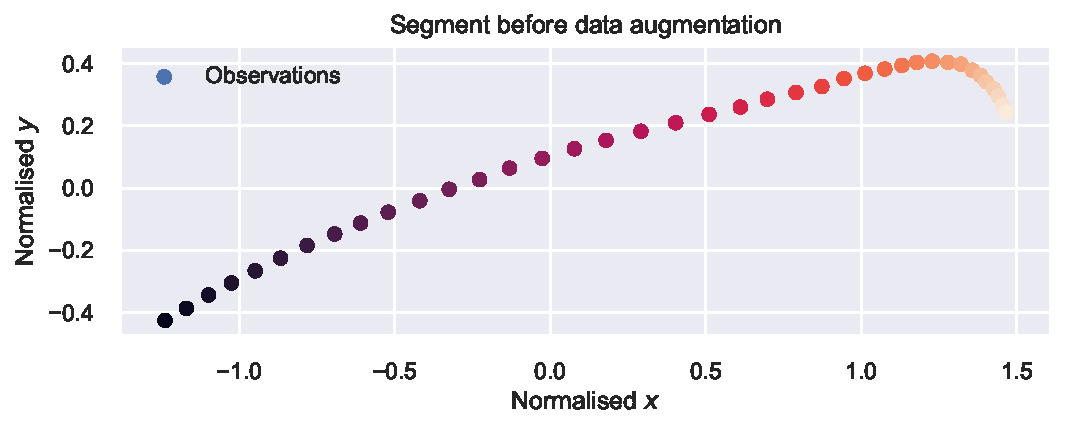
\includegraphics[scale=0.48,width=\textwidth]{data-augmentation-before}
    \caption{Spatial progression of a trajectory
      before data augmentation. Color indicate $\synchspace$ from
      dark ($\synchspace=0.0$) to bright ($\synchspace=1.0$).}\label{fig:traj-without-support-data}
  \end{minipage}
  \hspace{5pt}
  \begin{minipage}{.46\textwidth}
    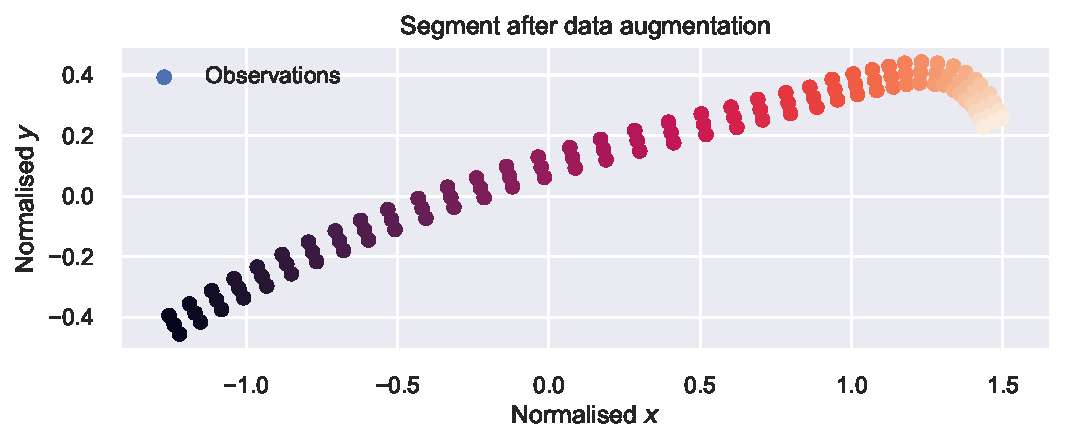
\includegraphics[scale=0.5,width=\textwidth]{data-augmentation-after}
    \caption{Spatial progression of a trajectory
      after data augmentation. Color indicate $\synchspace$ from
      dark ($\synchspace=0.0$) to bright ($\synchspace=1.0$).}\label{fig:traj-with-support-data}
  \end{minipage}
\end{figure}

\begin{figure}
  \begin{minipage}{.46\textwidth}
    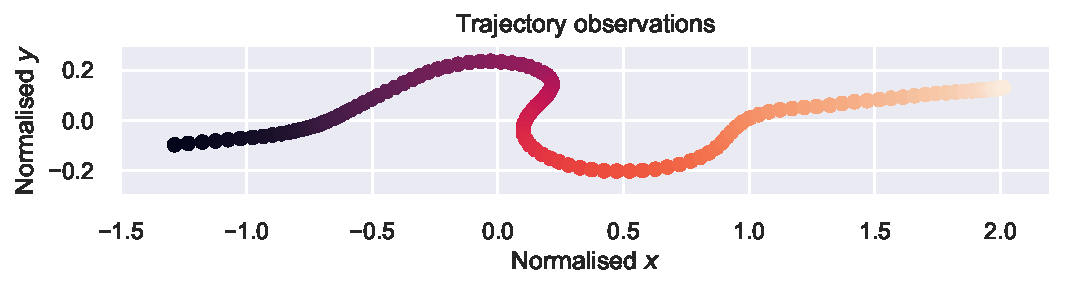
\includegraphics[scale=0.48,width=\textwidth]{trajectory-observation-example}
    \caption{Spatial observations of a segment. Colour indicate values
      of $\tau$, from brightdark ($\synchspace=0.0$) to bright ($\synchspace=1.0$).}\label{fig:seg-9-observations}
  \end{minipage}
  \hspace{5pt}
  \begin{minipage}{.46\textwidth}
    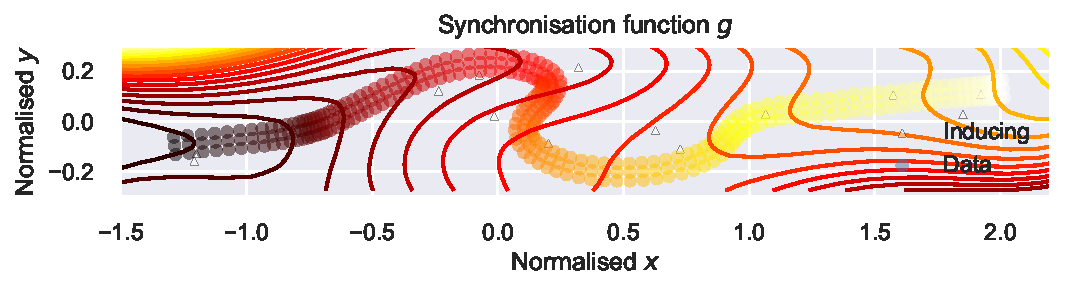
\includegraphics[scale=0.5,width=\textwidth]{synch-model-example}
    \caption{The learned synchronisation model $\synchf$. Colour indicate values
      of $\tau$, from brightdark ($\synchspace=0.0$) to bright ($\synchspace=1.0$).}\label{fig:seg-9-g}
  \end{minipage}
\end{figure}

\subsubsection{Handling Stand-stills}\label{sec:stop-compression}
Stand-stills causes an uneven spatial distribution of data. This is
prevented using stop compression, which aggregates observations in close proximity into a
single observation through averaging. Observations within a radius of
$\epsilon$ are clustered into a single observation with the mean value of
the clustered observations. An example of this is seen
Figure~\ref{fig:stop-compression-before} and
Figure~\ref{fig:stop-compression-after}. During evaluation $\epsilon=4$ metres was used. 
\begin{figure}
  \begin{minipage}{.46\textwidth}
    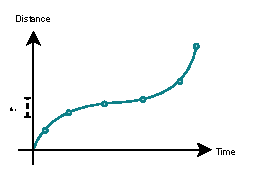
\includegraphics[scale=0.48,width=\textwidth]{stop-compression-before}
    \caption{Trajectory before stop compression. Observations are 
      approximately uniformly distributed temporally, but form a cluster
      much denser than the desired $\epsilon$ spatialy. }\label{fig:stop-compression-before}
  \end{minipage}
  \hspace{5pt} 
  \begin{minipage}{.46\textwidth}
    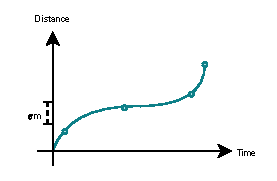
\includegraphics[scale=0.5,width=\textwidth]{stop-compression-after}
    \caption{Spatial progression of a trajectory
      after stop compression. Data which within a radius of $\epsilon$
      has been compressed so the resulting data is
      approximately uniformly distributed spatially.}\label{fig:stop-compression-after}
  \end{minipage}
\end{figure}

\subsection{Learning the Motion Pattern Model}
The motion pattern model of a single trajectory is defined by the family of
function $(\modelf_{p_x}, \modelf_{p_y}, \modelf_{v_x}, \modelf_{v_y})$
that map from $\synchspace$ to $\statespace$.
The uncertainty of these models depend on how the buses move and how
accurate sensors they are equipped with. Since traffic moves smoothly 
and modern sensors can measure position and velocity quite accurately, 
there is very little noise in these models, which leads to an undesirably low variance. 
This causes a motion pattern model to consider observations that are just a few
meters away to be highly unlikely, which means that it will never be
able to confidently predict a likely motion pattern for observed data.
This issue is addressed by defining \textit{pseudo-clusters} models,
which have desirable variance. 
A pseudo-cluster $\combinedf$ is created for each GP in the motion pattern
model. They are all created in the same way, and unless specifically
stated, $\combinedf$ can belong to any GP in a
motion pattern model. I.e. $\combinedf_{p_x}$ would belong to $\modelf_{p_x}$.
$\combinedf$ is modeled pont-wise as
$\combinedf(\synchslice) \sim \mathcal{N}(\mu(\synchslice), \sigma^2(\synchslice))$
for any point $\synchslice$ and for each state model
$\modelf_{p_x}, \modelf_{p_y}, \modelf_{v_x}, \modelf_{v_y}$. The
pseudo-cluster parameters $\mu(\synchslice), \sigma^2(\synchslice)$ are given by using the
\textit{combining formula}~\cite{Tiger2015Jul}
\begin{equation}
  \label{eq:combining-formula-mu}
  \mu(\tau^{*}) = \frac{\sum_{j=1}^{J}N_{j}\mu_j(\tau^{*})}{\sum_{j=1}^{J}N_j}
\end{equation}
\begin{equation}
  \label{eq:combining-formula-sigma}
  \sigma^2(\tau^{*}) =
  \frac{\sum_{j=1}^{J}N_{j}(\sigma^2_j(\tau^{*}) + \mu_j^2(\tau^{*}))}{\sum_{j=1}^{J}N_j}
\end{equation}
with uniform weights $N$ over two copies of $\modelf$, offset by
$\delta$ orthogonal to $\tau$. $\delta$ is a user-specified parameter
which controls what distance the model should consider close when
comparing trajectories. During evaluation $\delta=<TODO>$ was used. As is illustrated in Figure~\ref{fig:pseudo-cluster-before} and
Figure~\ref{fig:pseudo-cluster-after}, this creates a larger variance, 
which enables meaningful comparison of models.
\begin{figure}
  \begin{minipage}{.46\textwidth}
    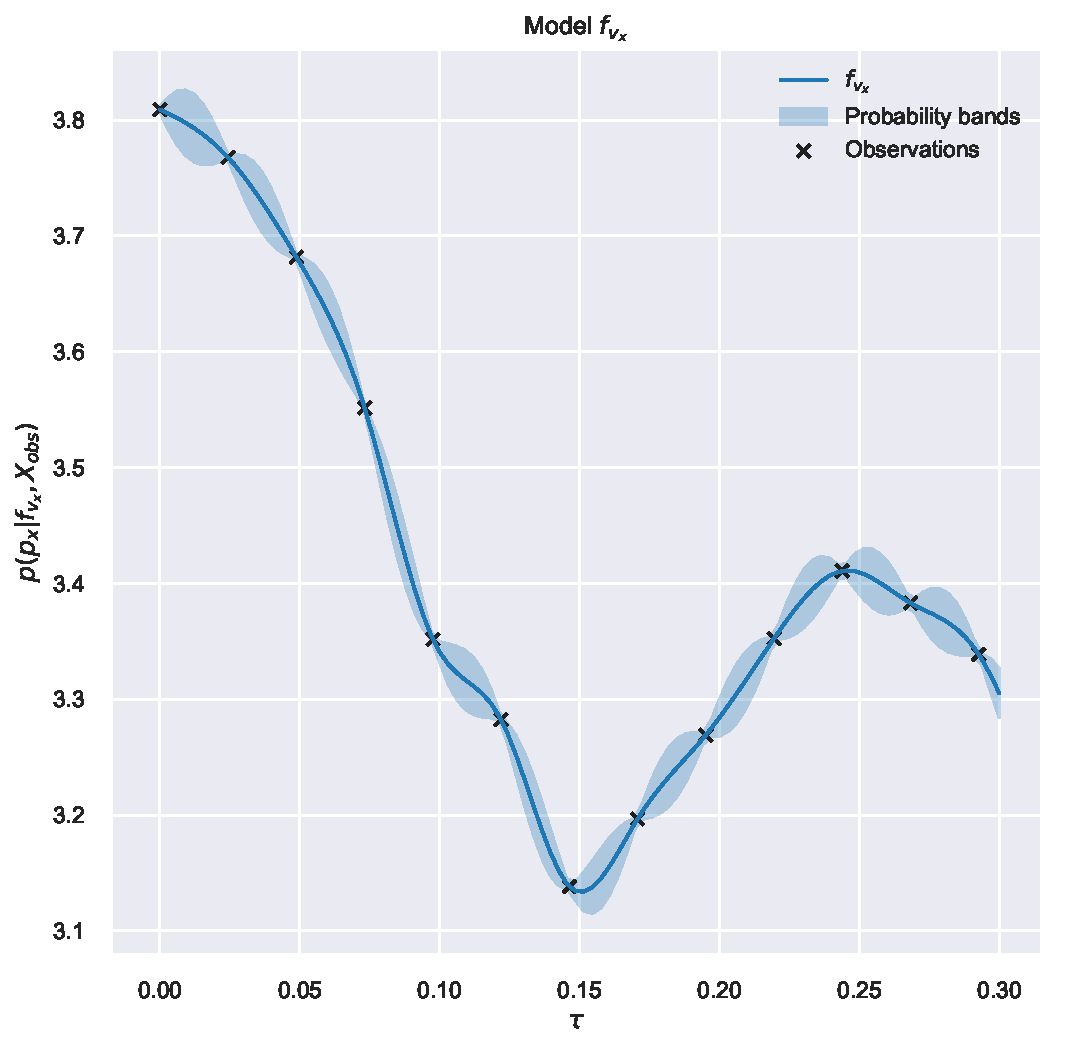
\includegraphics[scale=0.48,width=\textwidth]{pseudo-cluster-before}
    \caption{A state model fit on observation data. Trajectory data close-by
    will appear highly unlikely.}\label{fig:pseudo-cluster-before}
  \end{minipage}
  \hspace{5pt}
  \begin{minipage}{.46\textwidth}
    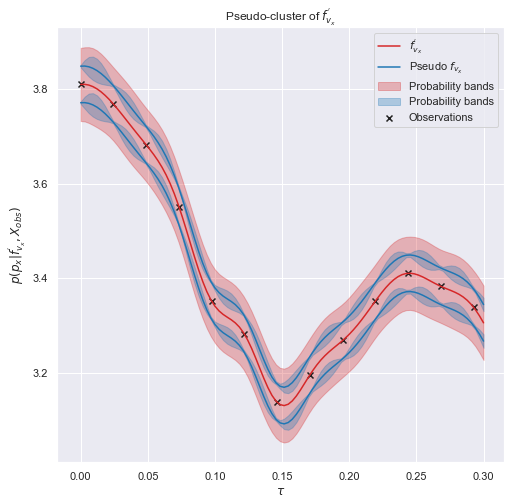
\includegraphics[scale=0.5,width=\textwidth]{pseudo-cluster-after}
    \caption{A state model fit on a pseudo-cluster. Trajectory data close-by
    will appear likely.}\label{fig:pseudo-cluster-after}
  \end{minipage}
\end{figure}

\section{Querying the model}
There are two queries that can be asked of the model. The first one is
arrival time prediction and the second is event detection. This
section addresses how both these queries are performed.

\subsection{Arrival Time Prediction}
The predicted arrival time for observation $\newobs$
is given by equation~\ref{eq:arrival-time-probability} for the most similar, 
or probable, model $\hat{\model}$. $\hat{\model}$ is given by Bayesian model 
selection with a uniform prior over all learned models
\begin{equation}
  \label{arrival-time-model-selection}
  \hat{\model} = \argmax_k
  \prob(\model_k \vert \stochobs = \newobs) =
  \prob(\stochobs = \newobs \vert \hyperparam_{k}, \model_k)
  \prob(\model_k) \propto
  \prob(\stochobs = \newobs \vert \hat{\hyperparam}_{k}, \model_k),
\end{equation}
where $\hat{\hyperparam}_{k}$ are the ML-estimated
hyper-parameters of corresponding model $\model_{k}$.
Given the uniform prior, the model which maximises the likelihood is
selected, which is equivalent with the model that maximises the log
likelihood, since the log function is monotonically increasing. The
model log likelihood is given by the sum of the log likelihood of the
pseudo-cluster of individual GP models
\begin{equation}
  \label{eq:model-log-likelihood}
  \begin{split}
    \log \prob(\stochobs_{k} = x \vert \hat{\hyperparam}_{k}, \model_k)  
    = & \log \prob(\stochobs_{k} = x \vert \combinedf^{(k)}_{p_x}, \stochobs_{obs} = x) \\
    + & \log \prob(\stochobs_{k} = x \vert \combinedf^{(k)}_{p_y}, \stochobs_{obs} = x) \\
    + & \log \prob(\stochobs_{k} = x \vert \combinedf^{(k)}_{v_x}, \stochobs_{obs} = x) \\
    + & \log \prob(\stochobs_{k} = x \vert \combinedf^{(k)}_{v_y}, \stochobs_{obs} = x).
  \end{split}
\end{equation}
where the log likelihoods of pseudo-clusters are given
by equation~\ref{eq:gp-log-likelihood}. An illustration of model
probabilities computed in this way can be
seen in Figure~\ref{fig:model-probability}. Figure~\ref{fig:state-model} 
shows trajectory models that are presented with new
observations, together with the corresponding model
probabilities in Figure~\ref{fig:state-model-probabilities}.
\begin{figure}
  \centering
  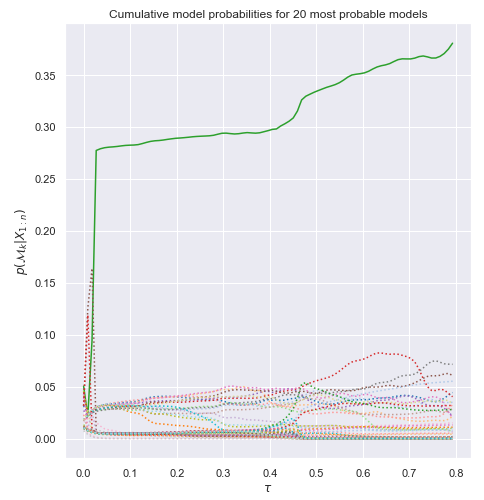
\includegraphics[scale=0.6]{model-probability}
  \caption{Plots of trajectory model probabilities from observed data.
    The model quickly identifies the true model, indicated by the
    solid line.}\label{fig:model-probability}
\end{figure}
\begin{figure}
  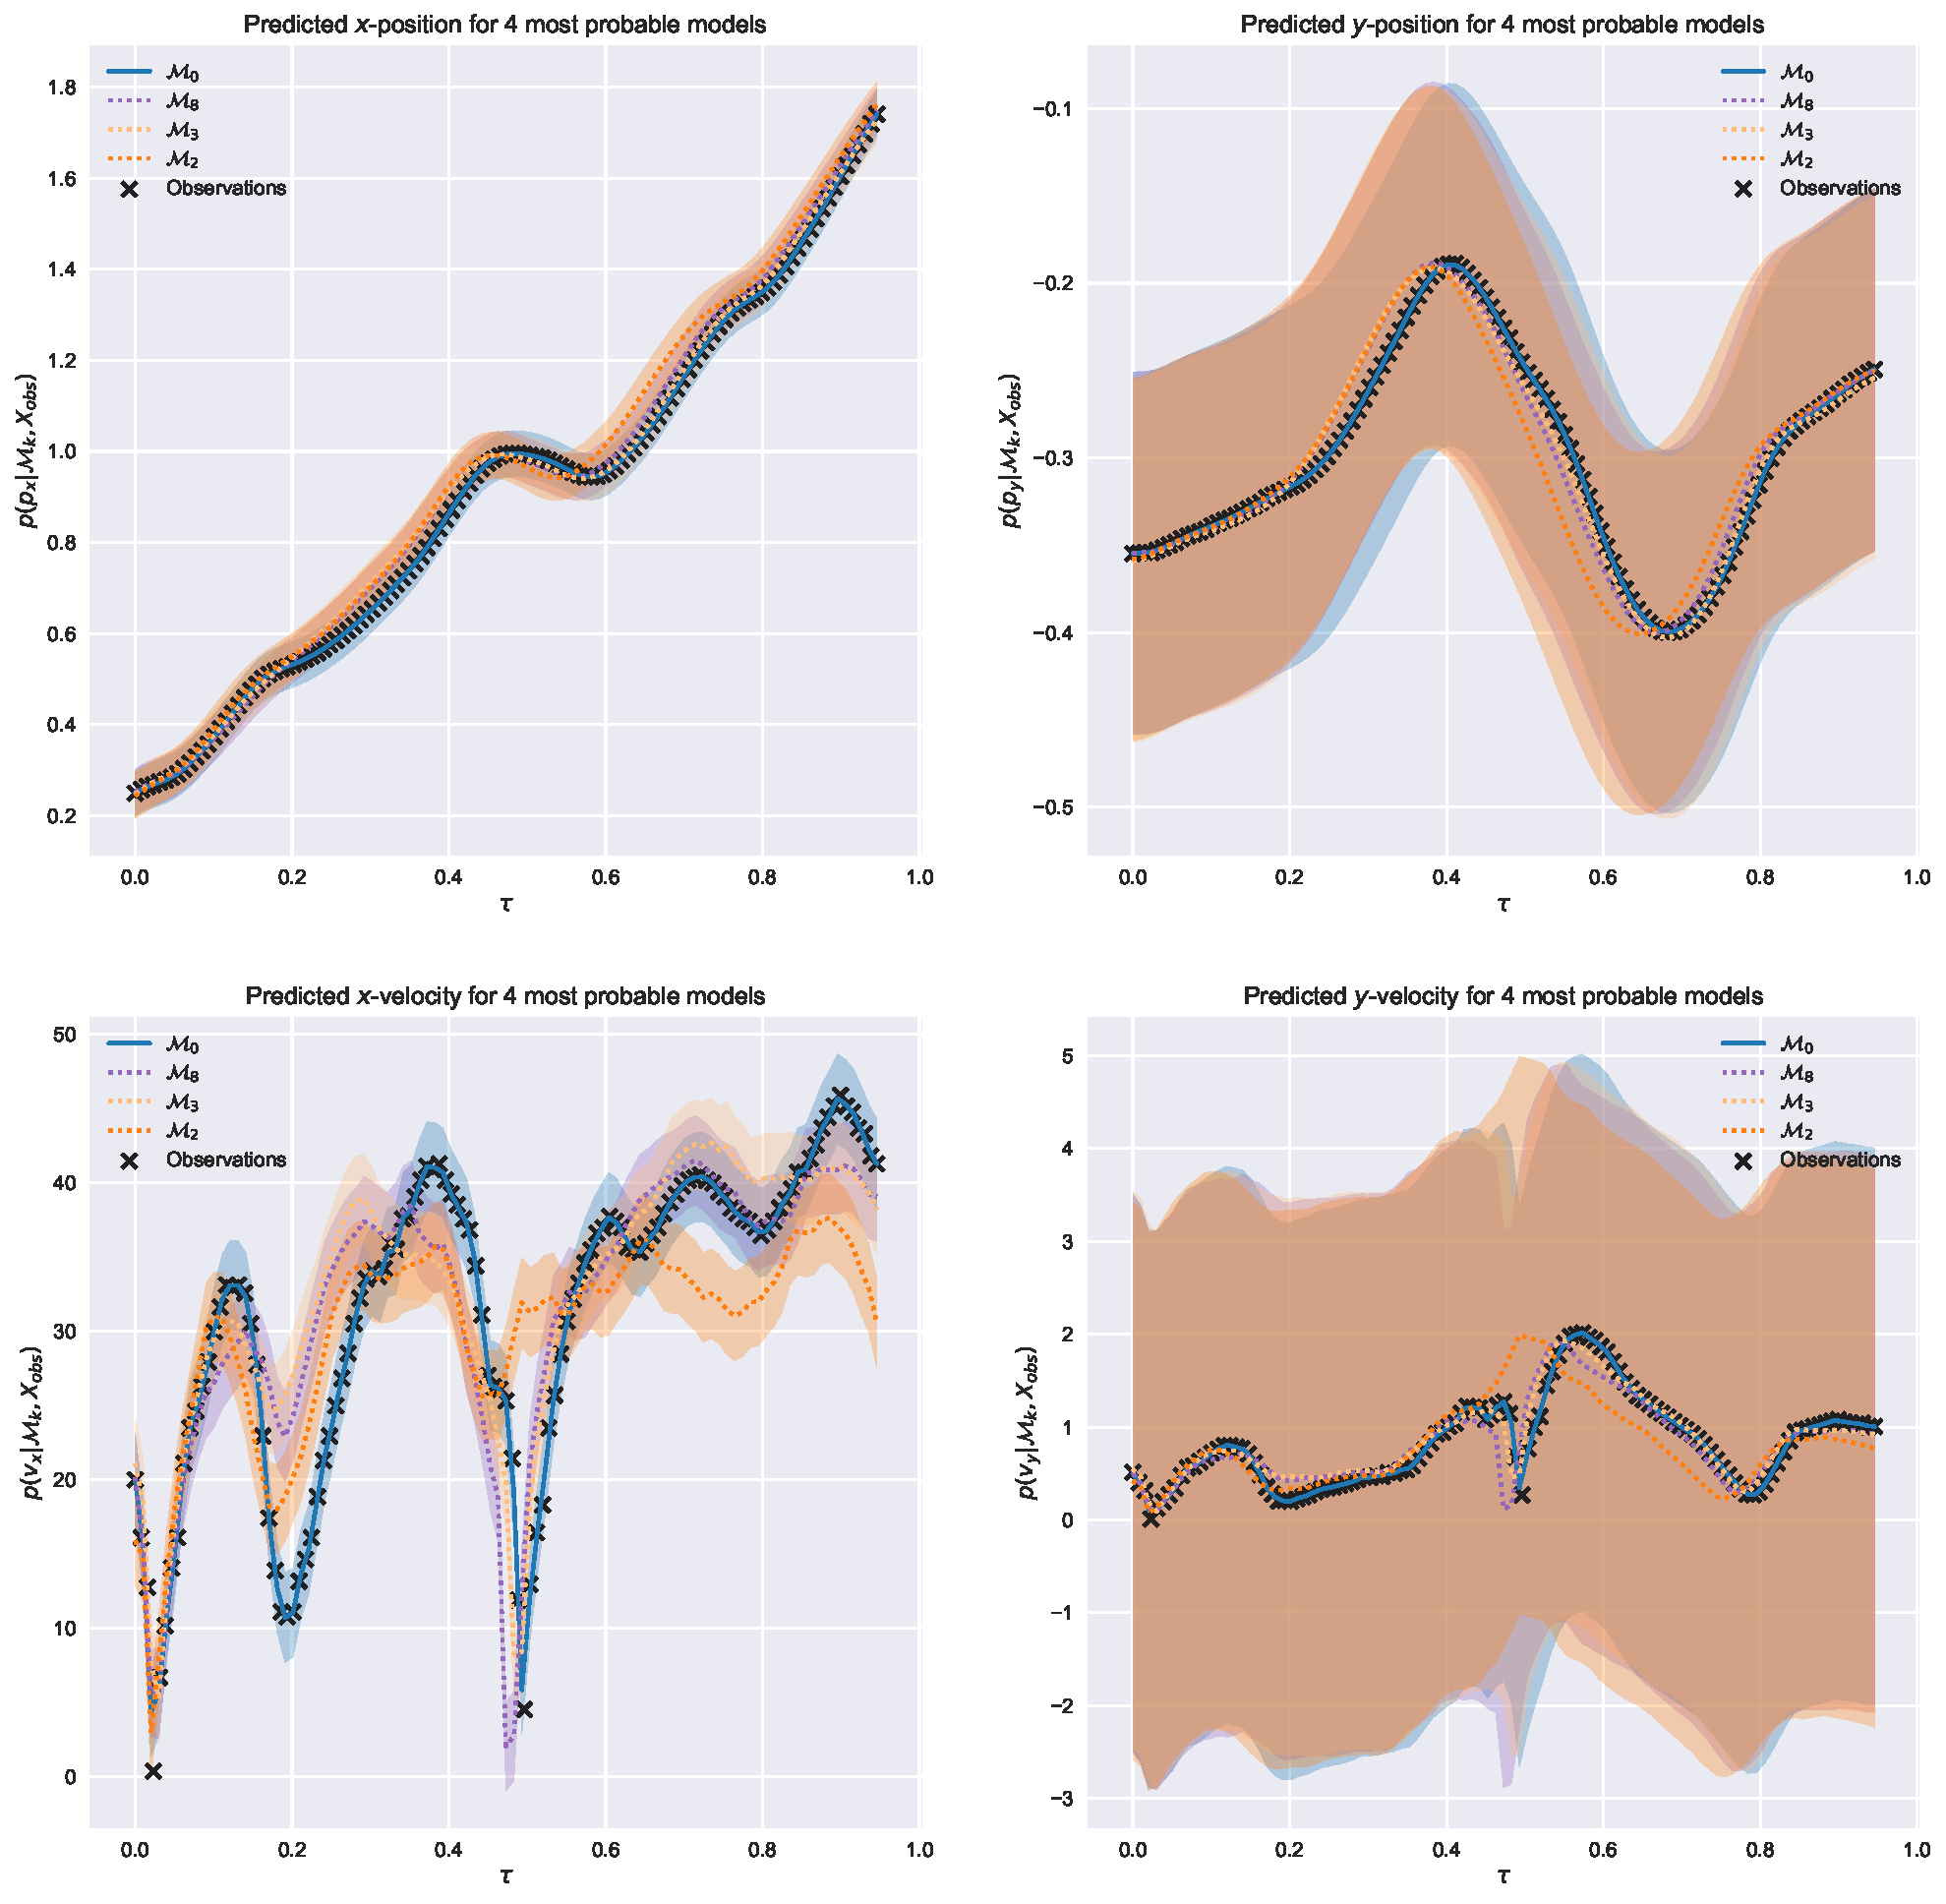
\includegraphics[scale=0.3,width=\textwidth]{model-example}
  \caption{Plots of state models mean functions
    and probability bands for different $\model_{k}$.}\label{fig:state-model}
\end{figure}
\begin{figure}
  \includegraphics[scale=0.3,width=\textwidth]{model-probabilities}
  \caption{Plots of the model probabilities for each state model. The model
    places high probability on the true model. It is able to identify
    the true model solely from velocity. Since all motions
    patterns are recorded on the same road road, they are incredibly
    similar and so the spatial information does not
    convey any information, as indicated by the noisy plots.}\label{fig:state-model-probabilities}
\end{figure}
While predicting arrival time through equation~\ref{eq:arrival-time-probability} gives the correct mean, the
variance in the predictive distribution 
$\arrtime_{k} \sim \mathcal{N}(\mu_{\predf_k}, \sigma_{\predf_k})$
only considers the uncertainty in $\predf_k$. This is very optimistic,
since the uncertainty in arrival time depend on variance in 
velocity in the motion patterns to a great extent.
The uncertainty is more accurately modeled as 
$\sigma_{t_k} = \sigma_{\predf_k} + \sigma_{mp}$ where the addition $\sigma_{mp}$ is 
the motion pattern uncertainty given by integrating over
the probability bands of $f_{v_x}$ and $f_{v_y}$
\begin{equation}
  \label{eq:motion-pattern-variance-integral}
    \sigma_{mp} = \int_{\synchapsce} 2\sigma_{v_x}(\synchspace) + 2\sigma_{v_x}(\synchspace) d\synchspace
\end{equation}
where $\sigma_{v_x}(\synchspace)$ and $\sigma_{v_y}(\synchspace)$ are
given by the square root of the pseudo cluster variances from
equation~\ref{eq:combining-formula-sigma} for velocity models $\combinedf^{(k)}_{v_x}$
and $\combinedf^{(k)}_{v_y}$.

$$ \int_{\tau_0}^{\tau_1} 2\sigma(\tau) d\tau = \int_{\tau_0}^{\tau_1}
2\sigma d\tau  = 2\sigma \int_{\tau_0}^{\tau_1} d\tau =
2\sigma(\tau_1 - \tau_0)$$
%% The arrival time predictions are modeled as a Mixture of Gaussian
%% Processes (MoGP), where each previously observed model $\model_{k}$ induce a component. The
%% model predicts remaining time until arrival $\arrtime$ through the mixture
%% \begin{equation}
%%   \label{eq:arrival-time-mixture}
%%   \prob(\arrtime \vert \stochobs_{k} = \obs, \stochobs_{obs} = \obs) = 
%%   \sum_{k}\prob(\arrtime_{k} \vert \stochobs_{obs} = \obs, \model_{k})
%%   \prob(\model_{k} \vert \stochobs_{k} = \obs, \stochobs_{obs} = \obs),
%% \end{equation}
%% where the components $\prob(\arrtime_{k} \vert \stochobs_{obs} = \obs,
%% \model_{k})$ are given by equation~\ref{eq:arrival-time-probability},
%% and the weights $\prob(\model_{k} \vert \stochobs_{k} = \obs, \stochobs_{obs} = \obs)$
%% are given by equation~\ref{eq:model-posterior-probability}. Since all
%% components are Gaussian, the distribution will have one mode for each component. The
%% actual arrival time prediction of the model is the largest mode.

% $P(\model^{(k)}_{synch})$, given by equation~\ref{eq:model-posterior}, 
% since they are trained on the same $\traj_{k}$. Since all components are Gaussian, 
% $P(\arrtime \vert \obs)$ will have one mode for each component. The
% point-estimate prediction of the model is taken to be the largest
% mode, corresponding to the mean prediction of the most probable model.

% \begin{figure}[H]
%   \begin{minipage}{.46\textwidth}
%     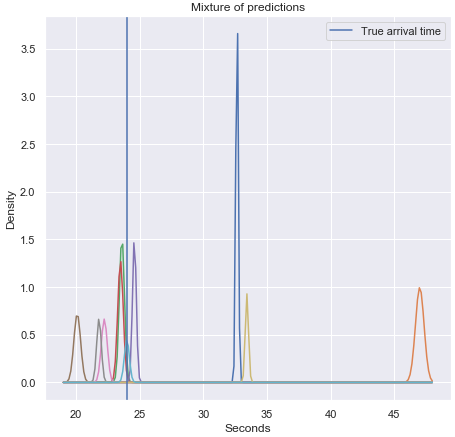
\includegraphics[width=\textwidth]{figures/mixture-start-of-traj.png}
%     \caption{Density of arrival time predictions at 
%       the start of a segment.}\label{fig:mixture-start-of-traj}
%   \end{minipage}
%   \hspace{5pt}
%   \begin{minipage}{.46\textwidth}
%     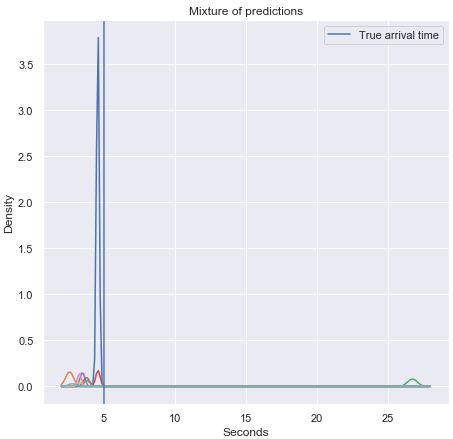
\includegraphics[width=\textwidth]{figures/mixture-end-of-traj.png}
%     \caption{Density of arrival time predictions at 
%       the end of a segment.}\label{fig:mixture-end-of-traj}
%   \end{minipage}
% \end{figure}

\subsection{Event Detection}
The problem of detecting events have not yet been investigated.

% A motion pattern representing a set of trajectory GPs can be though of as a GP as well. 
% This GP would capture the mean function of all
% underlying GPs, and their total variance. However, the implementation
% models one motion pattern for each trajectory, so the underlying set of 
% GPs is always a singleton $\{\modelf_k\}$. In addition, $\modelf_k$ has very
% small posterior variance since there is almost no noise.
% This results in a motion pattern with equally small posterior
% variance, and a likelihood for new observations which is close to zero
% for almost all trajectories, even those that are similar. This makes
% the likelihood meaningless as a similarity metric. To prevent this, a
% greater uncertainty is artificially created, by fixing the noise variance
% parameter $\sigma_n$ of the models to a higher value than would if it
% would have been estimated from data. This is illustrated in
% Figure~\ref{fig:too-small-variance} and Figure~\ref{fig:ok-variance}.
% \begin{figure}[H]
%   \begin{minipage}{.46\textwidth}
%     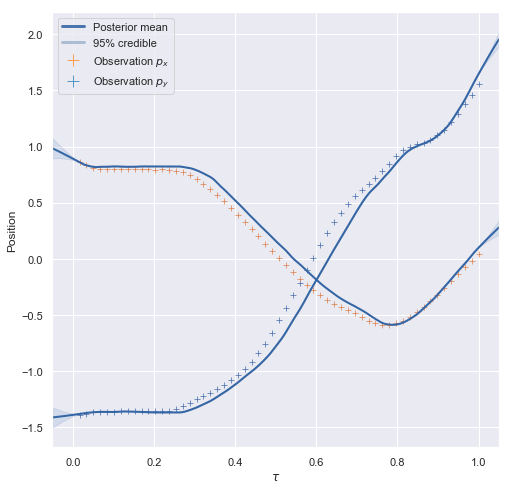
\includegraphics[width=\textwidth]{figures/too-low-variance}
%     \caption{GP posterior for for $x$ and $y$ coordinates, together with new
%       observations. The posterior variance is close to zero, so all
%       new data lies outside the 95\% credible interval and the
%       likelihood is very small. }\label{fig:too-small-variance}
%   \end{minipage}
%   \hspace{5pt}
%   \begin{minipage}{.46\textwidth}
%     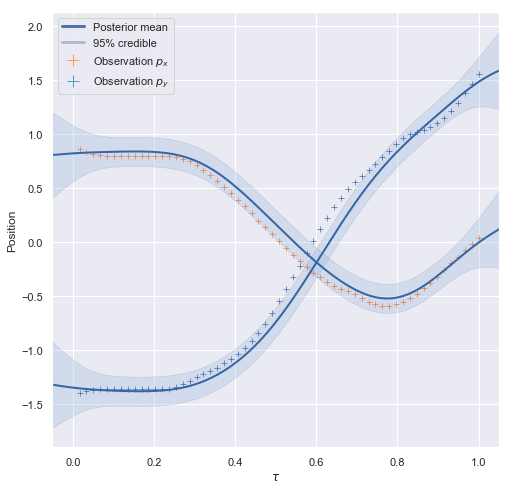
\includegraphics[width=\textwidth]{figures/ok-variance}
%     \caption{GP posterior for for $x$ and $y$ coordinates, together with new
%       observations. The posterior variance has been artificially increased, so the
%       new data is mainly inside the 95\% credible interval and
%       consequently is more likely.}\label{fig:ok-variance}
%   \end{minipage}
% \end{figure}

\section{System Implementation Details}
This section describes the implementation details of the system and
how data was processed. The GP implementations were done in Python, using the GPy
framework~\cite{gpy2014}, which uses the BFGS algorithm~\cite{fletcher2013practical} for
optimising $\hyperparam$. The database
PostgreSQL~\cite{BibEntry2019Feb} was used for storing trained GPs.

The integrals in equation~\ref{eq:motion-pattern-variance-integral}
were computed by approximating them by <inte klar här, osäker>
%% \begin{equation}
%%   \sigma_{mp} \approx \sum_{\synchspace=0.0}^{1.0}
%%   \left(2\sigma_{v_x}(\synchspace) + 2\sigma_{v_y}(\synchspace)\right)
%% \end{equation}
%%  with a step size of $0.02$.



% \subsection{Prediction Model}
% Predicting arrival time can be seen as learning the remaining time of
% a segment given a certain position $(p_x, p_y)$. However, modeling it
% as simple as as function of $(p_x, p_y)$ directly would assume that 
% every trajectory passes the exact same positions. A better model is $\arrtime_{k}
% = \predf_{k}(\synchspace)$, for arrival time $\arrtime_{k}$, 
% which instead depends on progression. Since the
% progression represents similar trajectories and not a single one, this
% model generalises much better. Assuming that $\arrtime_{k} \sim
% \mathcal{N}(\mu_{\arrtime_{k}}, \Sigma_{\arrtime_{k}})$, a GP can model
% $\predf_{k}$, which gives
% \begin{equation}
%   \label{eq:arrival-time-probability}
%   \prob(\arrtime_{k} \vert \stochobs_{obs} = \newobs, \model_k) 
%   = \int \prob(\arrtime_{k} \vert \synchspace,
%   \model_{k}) \prob(\synchspace \vert \stochobs_{obs} 
%   = \newobs, \model_{k}) d\synchspace,
% \end{equation}
% where $\prob(\arrtime_{k} \vert \stochobs_{obs} = \newobs, \model_k)$ 
% and $\prob(\synchspace  \vert \stochobs_{obs} = \newobs,
% \synchmodel_{k})$ are given by equations~\ref{eq:gp},~\ref{eq:gp-mean-function},
% and~\ref{eq:gp-covariance-function} for the GPs modeling
% $\predf_{k}$ and $\synchf_{k}$ respectively.

% %extending the synchronisation model to the \textit{trajectory model}
% %$\model_{k} = (\modelf_{k}, \synchf_{k}, \predf_{k})$, illustrated in Figure~\ref{fig:trajectory-model}.
% \begin{figure}
%   \centering
%   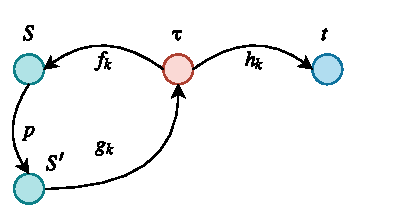
\includegraphics[scale=1.5]{trajectory-model}
%   \caption{An illustration of the trajectory model, which models
%     current state $\statespace$ and time left $\arrtime$ as functions of
%     progress $\synchspace$. $P$ denotes orthogonal projection from $\statespace
%     = (p_x, p_y, v_x, v_y)$, to $\posspace = (p_x, p_y)$.}\label{fig:trajectory-model}
% \end{figure}
